% (C) Marc Lijour, 2016-2017 
% Licensed under a Creative Commons License BY-SA
% https://creativecommons.org/licenses/by-sa/2.5/ca/
% Presentation for the Small Business Digitization Initiative (SBDI) training program
% see http://www.ictc-ctic.ca/small-business-digitization-initiative/ 
% authored by Marc Lijour, December 2016
% for the session running from January 2017 to September 2017
% 
% ======================================================================================================
%                                   GLOBAL COMPETITION - MACROECONOMIC FORCES
% ======================================================================================================
\section{Global Competition}
% --------------------- Currencies --------------------------
\subsection{Currency Competition}
\frame{
	\frametitle{Global Competition}
	\framesubtitle{Purchasing Power Parity (PPP)}
	\begin{itemize}
		\item Idea that a basket of common goods would have the same pricing value across countries and currencies
		\pause
		\item Assumptions:
			\begin{itemize}
				\item no transaction cost (currency exchange)
		\pause
				\item no trade barriers
			\end{itemize}
		\pause
		\item Useful to think about:
			\begin{itemize}
				\item Arbitrage
		\pause
				\item Undervaluation and overvaluation due to market expectation (e.g. US President Trump \& Mexico)
		\pause
				\item Policies such as currency fluctuation and trade barriers
			\end{itemize}
	\end{itemize}
}

\frame{
	\frametitle{Global Competition}
	\framesubtitle{Currency Valuation: \href{http://www.economist.com/content/big-mac-index}{The Big Mac Index}}
	% Discuss: it does not take into account labor cost
	\begin{figure}
	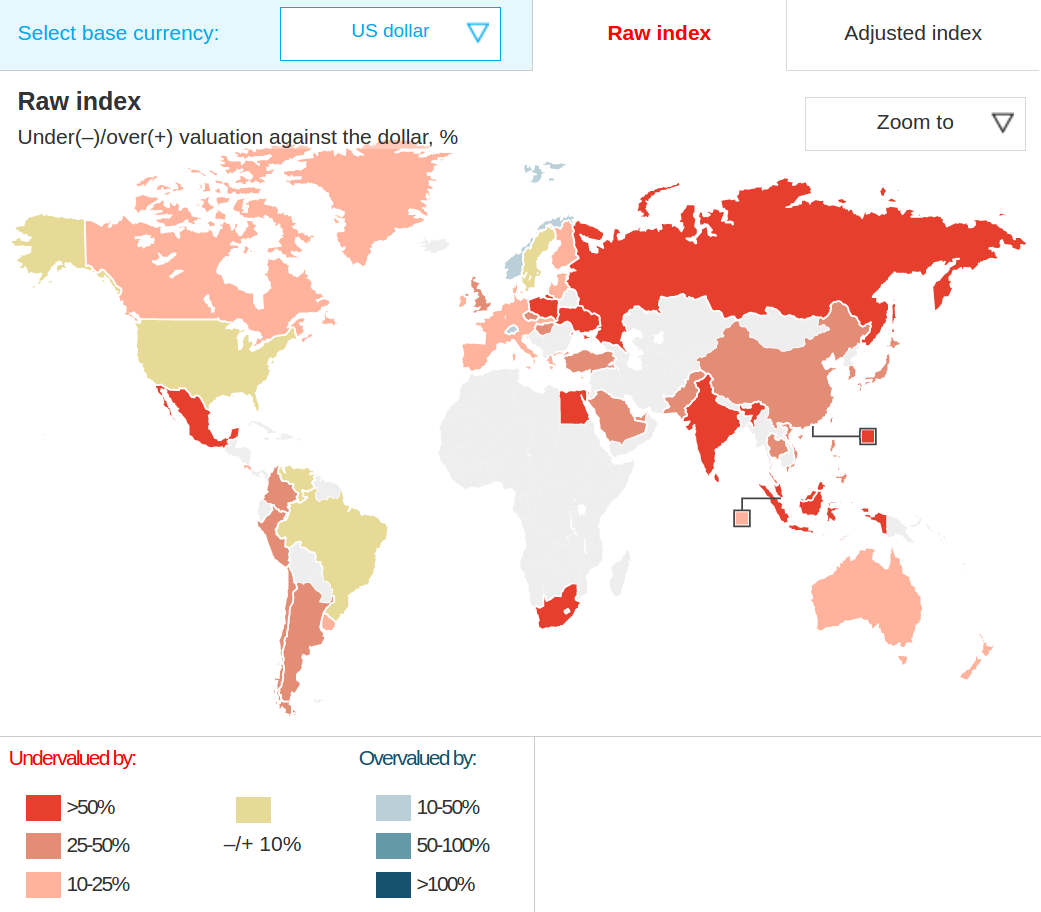
\includegraphics[height=7.5cm]{../pics/big-mac-index}
	\end{figure}
}

% --------------------- Trade Barriers --------------------------
\subsection{Trade Barriers}
\frame{
	\frametitle{Global Competition}
	\framesubtitle{Tariffs}
	\begin{itemize}
		\item Tax on the circulation of goods
		\pause
		\item See Canada Border Services Agency \href{http://www.cbsa-asfc.gc.ca/trade-commerce/tariff-tarif/2017/menu-eng.html}{Customs Tariff 2017}
		\pause
		\item Countries set their own policies, alone or in association (e.g. NAFTA, TPP, CETA)
		\pause
		\item Policies derive from political viewpoints (changing over time), for example
		\pause
			\begin{itemize}
				\item Canada cuts \$48M in tariffs on food ingredients to boost manufacturing, as \href{http://www.cbc.ca/news/politics/food-ingredient-tariff-cuts-1.3942870}{reported on CBC (January 20, 2017)}
		\pause
				\item US President Trumps threatened German car makers with a 35\% import tariff, as \href{http://business.financialpost.com/news/transportation/trump-threatens-german-carmakers-with-35-u-s-import-tariff}{reported on the Financial Post (January 16, 2017)}
			\end{itemize}
		\pause
		\item Impact on the Manufacturing Industry, Global Supply Chain, Foreign Investment, Currencies\ldots
	\end{itemize}
}

\frame{
	\frametitle{Global Competition}
	\framesubtitle{Non-Tariff Barriers}
	\begin{itemize}
		\item Circulation of staff delivering services across borders
		\pause
		\item Licensing (e.g. cryptography)
		\pause
		\item Standards
		\pause
		\item Quotas
		\pause
		\item Labeling and Packaging conditions
		\pause
		\item Intellectual Property Laws (e.g. patents)
		\pause
		\item Protected Designation of Origin (e.g. Champagne, Feta cheese)
	\end{itemize}
}

\subsection{Fiscal Policies}
\frame{
	\frametitle{Global Competition}
	\framesubtitle{Corporate Tax Rates}
	\begin{figure}
	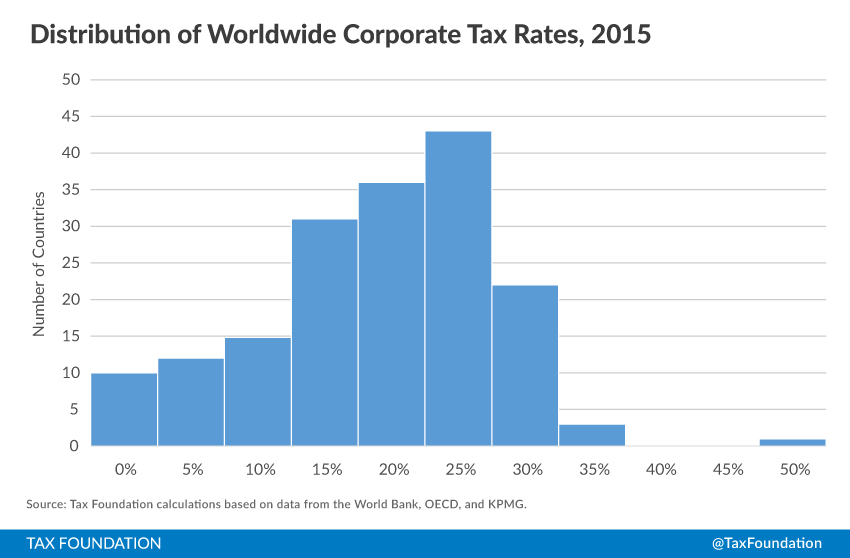
\includegraphics[height=7.5cm]{../pics/taxFoundation2015-worldwide-taxrates}
	\end{figure}
}

\frame{
	\frametitle{Global Competition}
	\framesubtitle{Corporate Income Tax Rates Competition (G7 Top 3 from \href{http://www.investinontario.com/spotlights/canada-ranks-1st-g7-corporate-tax-rate-and-cost-competitiveness}{KPMG, 2016})}
	\begin{figure}
	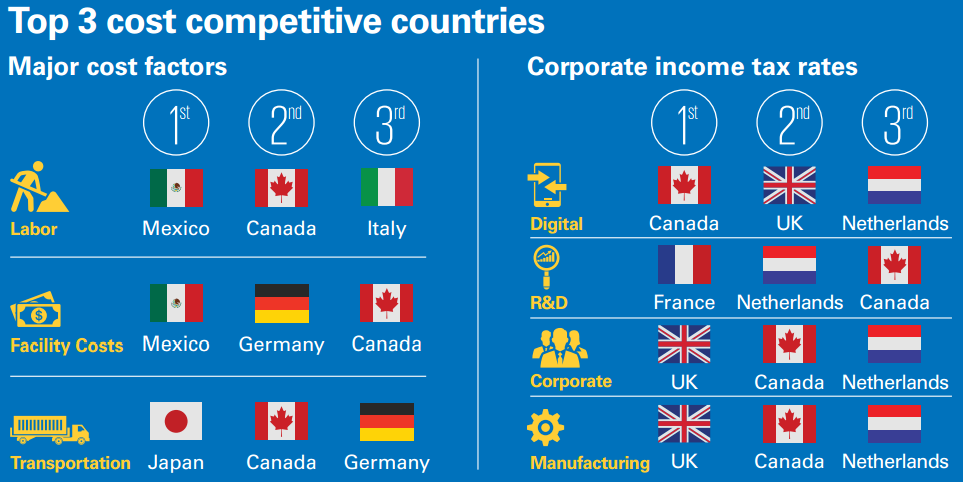
\includegraphics[width=11.5cm]{../pics/KPMG2016-top3-competitive-countries}
	\end{figure}
}

\subsection{Competitiveness Rankings}
\frame{
	\frametitle{Global Competition}
	\framesubtitle{Countries with the lowest business cost (G7 Top 10 from \href{http://www.investinontario.com/spotlights/canada-ranks-1st-g7-corporate-tax-rate-and-cost-competitiveness}{KPMG, 2016})}
	\begin{figure}
	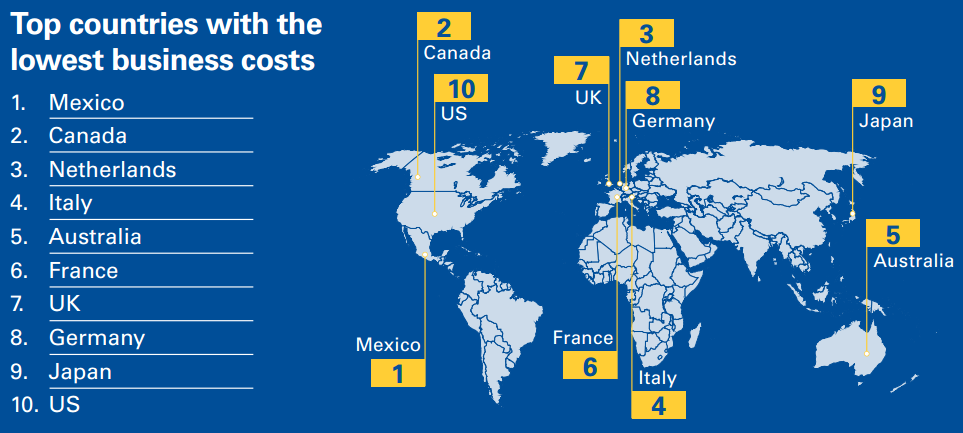
\includegraphics[width=11.5cm]{../pics/KPMG2016-top10-countries-wlow-bizcosts}
	\end{figure}
}

\frame{
	\frametitle{Global Competition}
	\framesubtitle{Business Cost Advantage: Greater Toronto vs USA (York Region, 2016)}
	\begin{figure}
	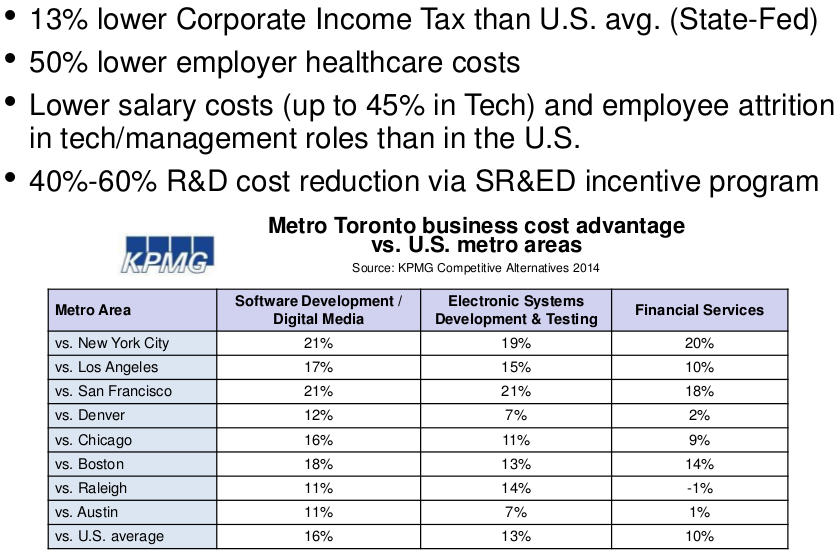
\includegraphics[height=7.5cm]{../pics/York-GTA-cost-advantage-vs-USA}
	\end{figure}
}

\frame{
	\frametitle{Global Competition}
	\framesubtitle{Manufacturing Competitiveness (Global Top 10 from \href{https://www2.deloitte.com/global/en/pages/manufacturing/articles/global-manufacturing-competitiveness-index.html}{Deloitte, 2016})}
	\begin{figure}
	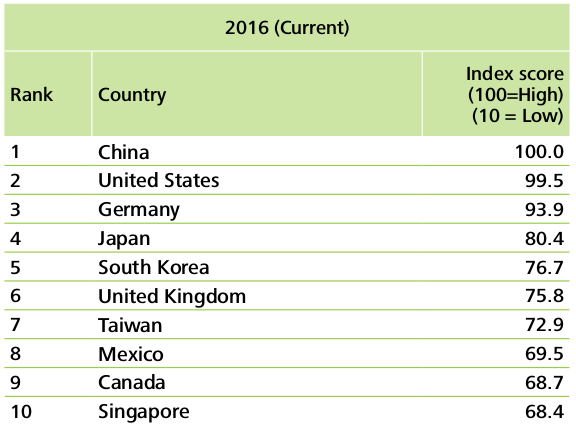
\includegraphics[height=7.5cm]{../pics/deloitte2016-top10-manufacturing-competitiveness}
	\end{figure}
}

\frame{
	\frametitle{Global Competition}
	\framesubtitle{Global Competitiveness Index (Global Top 15 from \href{http://www3.weforum.org/docs/gcr/2015-2016/Global_Competitiveness_Report_2015-2016.pdf}{World Economic Forum, 2016})}
	\begin{figure}
	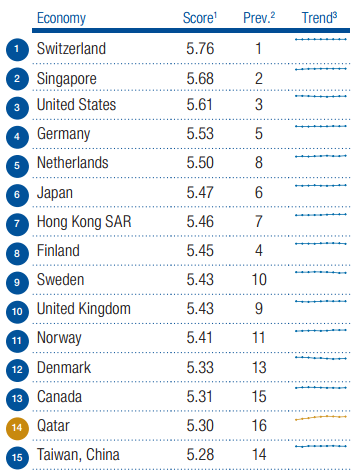
\includegraphics[height=7.5cm]{../pics/wef2016-global-competitiveness-index}
	\end{figure}
}

\frame{
	\frametitle{Global Competition}
	\framesubtitle{VC Money Invested in North American Cities (Thomson Reuters, 2016)} % First nine months of 2016 
	\begin{figure}
	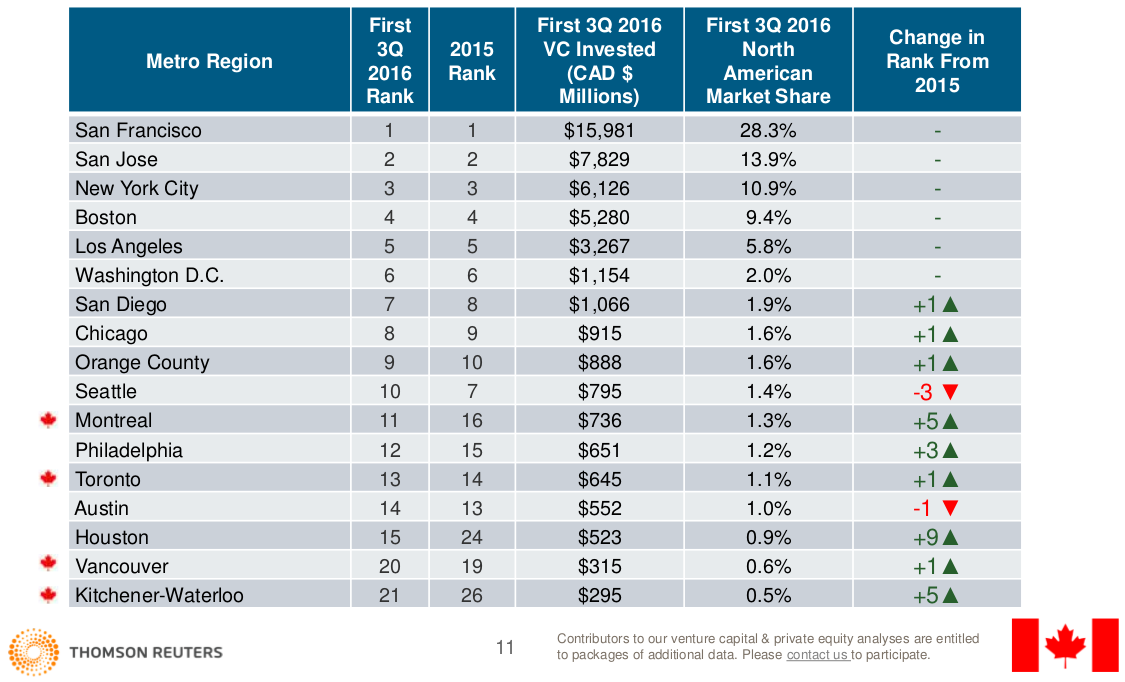
\includegraphics[height=7.4cm]{../pics/thomsonreuters2016-VC-funding-NA}
	\end{figure}
}

\frame{
	\frametitle{Global Competition}
	\framesubtitle{ICT Cluster Density across Canada (York Region, 2016)}
	\begin{figure}
	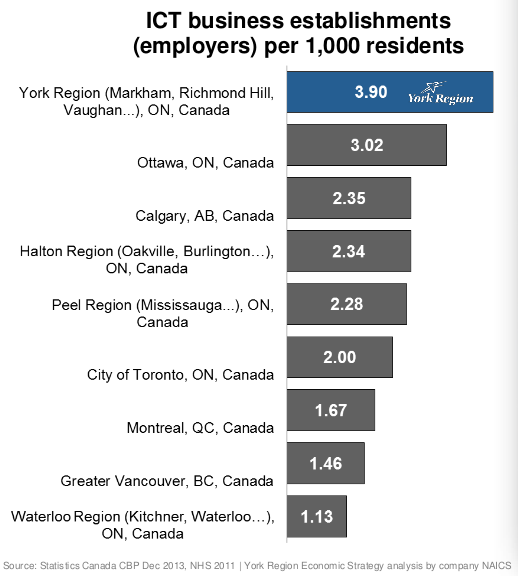
\includegraphics[height=7.5cm]{../pics/York-Canada-ICT-business-density}
	\end{figure}
}

\frame{
	\frametitle{Global Competition}
	\framesubtitle{Size of Ontario ICT Clusters (York Region, 2016)}
	\begin{figure}
	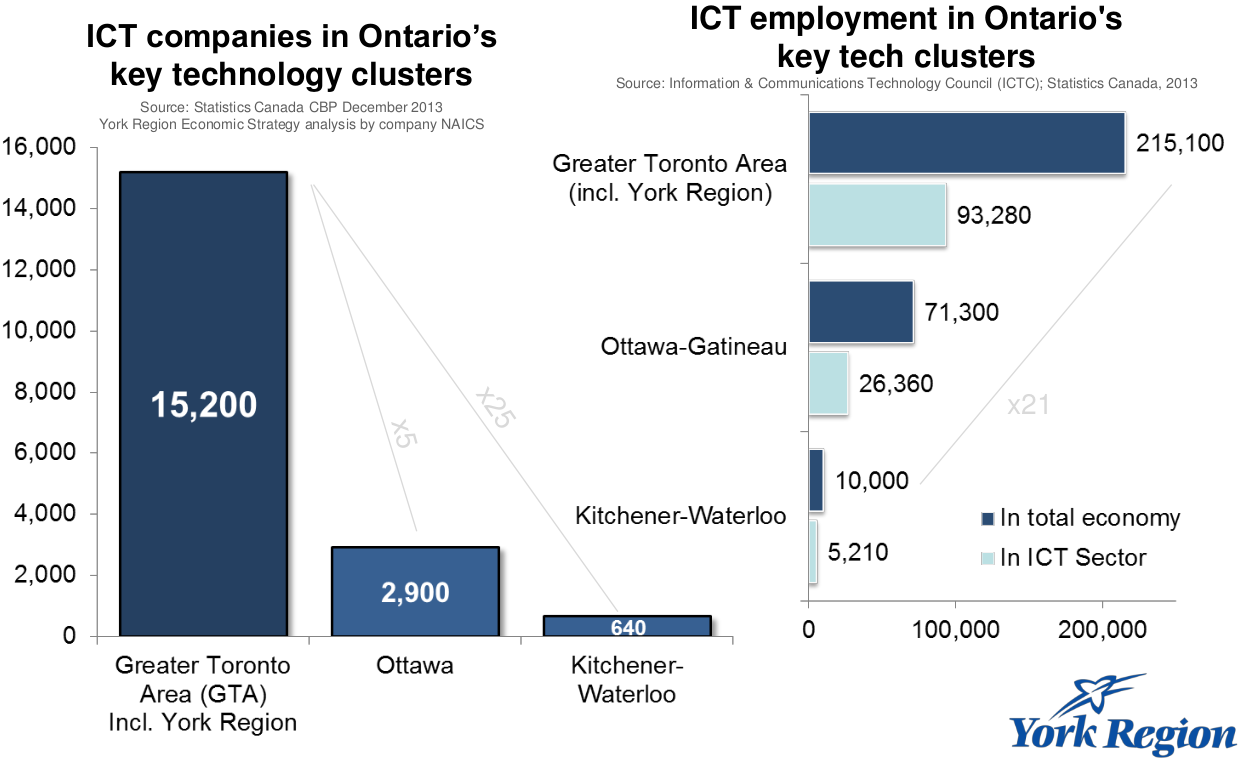
\includegraphics[height=7.4cm]{../pics/York-ICT-cluster-size}
	\end{figure}
}

\frame{
	\frametitle{Global Competition}
	\framesubtitle{Top Canadian Cities by Diversification (\href{https://techtoronto.org/Report2016/}{TechTO, 2016})}
	\begin{figure}
	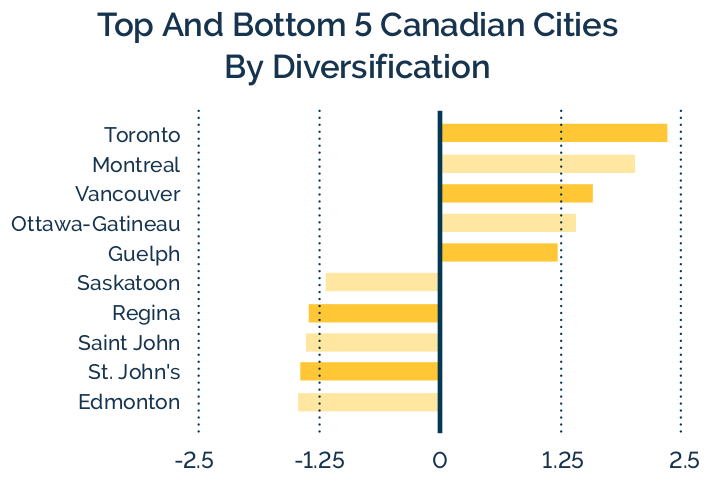
\includegraphics[height=6cm]{../pics/TechTO2016-Top-Canadian-Cities-by-Diversification}
	\end{figure}
}

\frame{
	\frametitle{Global Competition}
	\framesubtitle{References}
	% keyword refers to bib file: references-KEYWORD.bib, and to the Tex file: section-KEYWORD.tex
	\printbibliography[keyword=global-competition]
}

